% Finalizado 
\chapter{Desarrollo}
A continuación, se explicará el código del motor. Se detallará cómo se ha añadido cada módulo de simulación dentro de la arquitectura global. El objetivo es que la GPU tenga todo el ciclo de vida de los puntos. Con esto se evita el excesivo intercambio de datos entre el procesador principal y la memoria de vídeo (VRAM). El resultado es una mejora en el rendimiento del motor gráfico.

En las siguientes páginas se detallará la compilación de shaders en GLSL y la configuración de las pipelines gráficas. Asimismo, se describirá el proceso de reestructuración del flujo monolítico heredado del código base, optando por el uso de comandos asíncronos para lograr un diseño más robusto. Finalmente, se expondrán los fundamentos matemáticos subyacentes a la simulación de agua, fuego y humo.

\section{Creación de la pipeline de Computación}

El propósito principal es simular dinámicas físicas complejas, lo que implica procesar millones de elementos simultáneamente en pantalla. Para conseguir este propósito fue necesario diseñar una arquitectura paralela desde cero (\textit{Compute Pipeline}) basada en la API Vulkan. Su función es procesar operaciones matemáticas directamente en la GPU, utilizando para ello los \textit{Compute Shaders}.

La gestión de este bloque de ejecución recae sobre la clase \texttt{GEComputeShader}, responsable de instanciar la pipeline, monitorizar los recursos y liberar la memoria al término de su ciclo de vida mediante destructores automáticos basados en el patrón de diseño RAII~\parencite{stroustrup2013cpp}. Por otro lado, el cálculo de la física recae sobre la clase \texttt{GEParticleSystem}. Este componente reserva la memoria en la tarjeta gráfica y despacha (\textit{dispatch}) los hilos de ejecución concurrentes.

\subsection{Integración con la pipeline de renderizado global}

Fue necesario acoplar esta estructura de procesamiento dentro del ciclo de vida del motor. Para ello se emplearon tres clases preexistentes: \texttt{GERenderingContext}, \texttt{GECommandContext} y \texttt{GEScene}. El desafío principal radicó en la sincronización de la memoria compartida evitando condiciones de carrera o bloqueos. La clave reside en el orden de ejecución: la GPU calcula inicialmente la nueva posición de cada partícula; posteriormente, la pipeline gráfica lee estos datos de memoria para efectuar el renderizado tridimensional. El flujo interno se describe a continuación:

El componente \texttt{GEScene} maneja el arranque. Llama a \texttt{GERenderingContext} y le proporciona los parámetros de los emisores de partículas usando el método \texttt{createParticlePipelineConfig}. Con este paso definimos qué variables procesa el \textit{Vertex Shader}. Enlazamos de forma directa cosas como la posición, la normal de la superficie, el color, el tamaño y la edad que acaba de calcular la GPU.

Anteriormente, \texttt{GECommandContext} solo almacenaba órdenes de dibujado simples. Ahora también encola llamadas de cómputo.                                           
Todos estos comandos se despachan antes de pintar la escena. Gracias a esto, la gráfica actualiza las físicas y muestra la imagen.

% -----------------------------------------
\subsection{Carga de los shaders de computación}

Arrancar la \textit{pipeline} requirió un trabajo exhaustivo con \texttt{GEGraphicsContext}. 
El reparto de recursos se lleva a cabo mediante la clase \texttt{GEDescriptorSet}. 
Además, reservamos la memoria de la tarjeta usando la clase \texttt{GEParticleBuffer} (véase la Figura~\ref{fig:geparticlebuffer_code}). 
Este componente maneja tanto \textit{Uniform Buffers} como \textit{Storage Buffers}.

\begin{figure}[!htbp]
    \centering
\begin{carbonbox}
class GEParticleBuffer
{
public:
    VkBuffer buffer;
    VkDeviceMemory memory;
    GEParticleBuffer(GEGraphicsContext* gc, size_t size, const void* data);
    void destroy(GEGraphicsContext* gc);
};
\end{carbonbox}
    \caption{Código fuente del archivo \texttt{GEParticleBuffer.h}.}
    \label{fig:geparticlebuffer_code}
\end{figure}

\noindent Los recursos se vinculan del siguiente modo:

\begin{itemize}
    \item \textbf{Carga del programa y \textit{pipeline}:} Inicialmente, se cargan los \textit{compute shaders} precompilados en formato SPIR-V. A continuación, se emplea la estructura \texttt{VkComputePipelineCreateInfo}, la cual permite referenciar directamente el punto de entrada (\texttt{"main"}) del \textit{shader}.
    
    \item \textbf{Organización de la memoria (\textit{Layout}):} Se utiliza \texttt{VkDescriptorSetLayout} para definir la interfaz de datos y las estructuras que recibe el \textit{shader}.
    
    \item \textbf{Vinculación de recursos:} La clase \texttt{GEDescriptorSet} vincula los bloques de memoria centrales de la simulación:
    \begin{itemize}
        \item \textbf{Búferes de almacenamiento (SSBO):} Se emplean dos búferes, \texttt{particlesIn} y \texttt{particlesOut}, implementando una estrategia de doble búfer\footnote{Técnica también conocida como \textit{Ping-Pong Buffer}, consistente en el uso de dos búferes alternativos para evitar condiciones de carrera: mientras uno actúa como origen de datos de lectura, el otro almacena los resultados de escritura en cada fotograma.}. El búfer de entrada suministra el estado del fotograma anterior, mientras que en el de salida se escriben los resultados del nuevo cálculo físico.
        
        \item \textbf{Búfer uniforme (UBO):} Actúa a nivel global bajo el identificador \texttt{params}. Su función es suministrar a la tarjeta gráfica las variables de entorno dependientes del tiempo, tales como el diferencial de tiempo (\texttt{deltaTime}), la posición del emisor o la aceleración gravitatoria.
    \end{itemize}
\end{itemize}


\subsection{Flujo de integración}

Tal como se ilustra en el esquema de bloques de la Figura \ref{fig:jerarquia_ejecucion}, la ejecución del motor sigue un orden secuencial. 
De esta forma, la aplicación cede la administración de dichos procesos a la escena.  
La escena se encarga de controlar el ejecutado y el ciclo de sus \textit{pipelines}. 

\begin{figure}[!htbp]
\centering
\begin{tikzpicture}[
    node distance=1.2cm,
    block/.style={
        rectangle, 
        draw=blue!70!black, 
        fill=blue!5, 
        thick, 
        text width=3.8cm, 
        align=center, 
        rounded corners=2pt,
        minimum height=0.9cm,
        font=\small\ttfamily
    },
    arrow/.style={
        -{Stealth[scale=1.2]}, 
        thick, 
        draw=gray!80!black
    },
    dashed_arrow/.style={
        -{Stealth[scale=1.2]}, 
        thick, 
        dashed,
        draw=blue!80!black
    }
]
    % Nivel 1: Nodo inicial
    \node [block] (app) {GEApplication};
    
    % Nivel 2: Nodo orquestador
    \node [block, below=of app] (scene) {GEScene};
    
    % Nivel 3: Ramas de bifurcación (Físicas y Gráficos)
    \node [block, below=1.3cm of scene, xshift=-3.5cm] (compute) {GEComputeShader};
    \node [block, below=1.3cm of scene, xshift=3.5cm] (render) {GERenderingContext};
    
    % Nivel 4: Ejecutores finales
    \node [block, below=of compute] (sys) {GEParticleSystem};
    \node [block, below=of render] (geom) {Geometría y Skybox};
    
    % Conexión vertical principal
    \draw [arrow] (app) -- (scene);
    
    % Bifurcación ortogonal desde la escena hacia las ramas
    \draw [arrow] (scene.south) -- ++(0,-0.6) -| (compute.north) node[near end, left, font=\scriptsize\sffamily] {Físicas};
    \draw [arrow] (scene.south) -- ++(0,-0.6) -| (render.north) node[near end, right, font=\scriptsize\sffamily] {Gráficos};
    
    % Continuación de las ramas hacia abajo
    \draw [arrow] (compute) -- (sys);
    \draw [arrow] (render) -- (geom);
    
    % Flecha de sincronización (Lectura de buffers) transversal
    \draw [dashed_arrow] (sys.east) -- (geom.west) node[midway, above, font=\scriptsize\sffamily, align=center] {Lectura de\\búferes (SSBO)};
    
\end{tikzpicture}
\caption{Diagrama de bloques de la jerarquía de ejecución del motor gráfico.}
\label{fig:jerarquia_ejecucion}
\end{figure}

Para lograr una integración fluida entre el cálculo de física y el renderizado gráfico, la
escena divide su flujo de trabajo en varias fases importantes:

\begin{itemize}
    \item \textbf{Gestión de actualizaciones lógicas e físicas:} La escena separa la actualización visual, que maneja los eventos de entrada y las matrices de la cámara, de la actualización física, que introduce un paso de tiempo fijo (fixed delta time) a los sistemas de partículas para asegurar un determinismo matemático.

    \item \textbf{Sincronización mediante barreras de memoria:} La GPU opera asíncronamente, por lo que integrar la información implica sincronizar las fases de cálculo e interpolación. Al grabar comandos con \texttt{recordComputeCommands}, la escena inserta barreras de memoria (\texttt{VkBufferMemoryBarrier}). Estas barreras aseguran que las operaciones de lectura y escritura sean coherentes, evitando que el \textit{Vertex Shader} consuma datos espaciales antes de que el \textit{Compute Shader} haya finalizado su escritura en memoria.             

    \item \textbf{Orquestación del renderizado:} En la última etapa del dibujo (drawGraphicsObjects), la
escena pasa suavemente de una pipeline a otra. Define claramente el orden de visión:
primero: Skybox; luego, modelos 3D y figuras; terminando por la combinación de los
descriptor y buffers generados durante el paso de procesamiento para ilustrar las partículas.
\end{itemize}



\subsection{Cambios en la estructura del motor}

La provisión de soporte para el cálculo matemático en la GPU hizo necesaria la reescritura de ciertas secciones del código base, empleando para ello diversas extensiones oficiales de Vulkan. A modo de clarificación, se resumen los cambios en la Tabla~\ref{tab:modificaciones}:

\begin{table}[h!]
\centering
\begin{tabular}{|p{3.5cm}|p{6cm}|p{6cm}|}
\hline
\multicolumn{3}{|c|}{\textbf{Comparativa de modificaciones estructurales en el motor gráfico}} \\ \hline
\textbf{Clase} & \textbf{Estado Original} & \textbf{Estado Modificado (TFG)} \\ \hline
\texttt{GEComputeShader} & No existía en el motor. & Creada para inicializar \texttt{VkPipeline} de cómputo, \textit{descriptor pools} y layouts específicos para \textit{compute}. \\ \hline
\texttt{GEParticleSystem} \newline \texttt{GEParticle} & No existía en el motor. & Implementadas para definir la estructura de datos física de la partícula y despachar hilos (\textit{workgroups}). \\ \hline
\texttt{GECommandContext} & Solo grababa comandos para \texttt{VK\_PIPELINE\_BIND\_POINT\_GRAPHICS}. & Extendida para soportar la grabación de comandos \textit{Compute} mediante el método \texttt{recordCommands}. \\ \hline
\texttt{GEScene} \newline \texttt{GEApplication} & Controlaban únicamente figuras geométricas estáticas u objetos indexados (\texttt{GEPiece}). & Añaden la gestión del ciclo \texttt{update} de simulaciones físicas en la GPU. \\ \hline
\end{tabular}
\caption{Comparativa de modificaciones estructurales en el motor gráfico.}
\label{tab:modificaciones}
\end{table}

Para materializar los cambios estructurales resumidos en la Tabla~\ref{tab:modificaciones}, se han incorporado nuevos componentes y estructuras al motor gráfico. En primer lugar, la gestión lógica y la manipulación de los búferes de memoria doble (\textit{double buffering}) de las partículas se delega en la clase principal \texttt{GEParticlesSystem} (véase la Figura~\ref{fig:geparticlessystem_code}).

\begin{figure}[!htbp]
    \centering
\begin{carbonbox}
class GEParticlesSystem {
protected:
    std::vector<GEParticle> particles;
    std::vector<uint16_t> indices;
    glm::mat4 location;
    GEMaterial material;
    GELight light;
    std::unique_ptr<GEParticleBuffer> pboA;
    std::unique_ptr<GEIndexBuffer> ibo;
    std::unique_ptr<GEUniformBuffer> transformBuffer;
    std::unique_ptr<GEUniformBuffer> materialBuffer;
    std::unique_ptr<GEUniformBuffer> lightBuffer;
    std::unique_ptr<GEDescriptorSet> dset;
    std::unique_ptr<GEParticleBuffer> pboB;
    GEEmitterParams emitterParams;
    std::unique_ptr<GEUniformBuffer> emitterParamsBuffer;
    float lastTime;
public:
    GEParticlesSystem();
    void initialize(GEGraphicsContext* gc, GERenderingContext* rc, GETexture* sceneTexture);
    void destroy(GEGraphicsContext* gc);
    void addCommands(VkCommandBuffer commandBuffer, VkPipelineLayout pipelineLayout, int index);
    void update(GEGraphicsContext* gc, uint32_t index, glm::mat4 view, glm::mat4 projection);
    void resetLocation();
    void setLocation(glm::mat4 m);
    glm::mat4 getLocation();
    void translate(glm::vec3 t);
    void rotate(float angle, glm::vec3 axis);
    void setMaterial(GEMaterial m);
    void setLight(GELight l);
    GEParticleBuffer* getParticlesBufferA();
    GEParticleBuffer* getParticlesBufferB();
    size_t getParticlesSize();
    uint32_t getParticlesCount();
    void addParticle(GEParticle p);
    VkDescriptorSet getDescriptorSet(int index);
    GEUniformBuffer* getEmitterParamsBuffer();
    void updatePhysics(GEGraphicsContext* gc, uint32_t index, float fixedDeltaTime);
};
\end{carbonbox}
    \caption{Código fuente del archivo \texttt{GEParticlesSystem.h}.}
    \label{fig:geparticlessystem_code}
\end{figure}


\begin{figure}[!htbp]
    \centering
\begin{carbonbox}
typedef struct alignas(16)
{
    glm::vec4 color;      
    glm::vec3 pos;        
    float size;           
    glm::vec3 norm;       
    int activeTTL;        
    float ttl;            
    float currentTtl;     
} GEParticle;
\end{carbonbox}
    \caption{Código fuente del archivo \texttt{GEParticle.h}.}
    \label{fig:geparticle_code}
\end{figure}

Cada partícula individual dentro del sistema físico se modela mediante la estructura de datos \texttt{GEParticle} (véase la Figura~\ref{fig:geparticle_code}). Esta estructura está explícitamente alineada en memoria a un límite de 16 bytes (\texttt{alignas(16)}) para garantizar la compatibilidad con el diseño de memoria (\textit{layout}) esperado por los shaders en la GPU.                    

\vspace{3\baselineskip}
Por último, para abstraer la carga, compilación en tiempo de ejecución y despacho de la pipeline de cómputo en Vulkan, se diseñó la clase de control \texttt{GEComputeShader} (véase la Figura~\ref{fig:gecomputeshader_code}), la cual se responsabiliza de registrar los comandos de cómputo asíncronos y despachar los bloques de hilos (\textit{workgroups}) en la GPU.                                 

\begin{figure}[!htbp]
    \centering
\begin{carbonbox}
class GEComputeShader{
public:
    VkPipeline pipeline;
    VkPipelineLayout layout;
    VkDescriptorSetLayout descriptorSetLayout;
    VkDescriptorPool descriptorPool;
    std::vector<std::vector<VkDescriptorSet>> systemDescriptorSets;
    GEComputeShader(GEGraphicsContext* gc, int shaderResource, uint32_t imageCount);
    int addParticleSystem(GEGraphicsContext* gc, uint32_t imageCount, GEParticlesSystem* particleSystem);
    void recordCommands(VkCommandBuffer cb, uint32_t systemIndex, uint32_t imageIndex, uint32_t groupCountX);
    void destroy(GEGraphicsContext* gc);
private:
    void createDescriptorSetLayout(GEGraphicsContext* gc);
    void createDescriptorSets(GEGraphicsContext* gc, uint32_t imageCount);
    void createComputePipeline(GEGraphicsContext* gc, int shaderResource);
    std::vector<char> getFileFromResource(int resource);
    VkShaderModule createShaderModule(GEGraphicsContext* gc, const std::vector<char>& code);
};
\end{carbonbox}
    \caption{Código fuente del archivo \texttt{GEComputeShader.h}.}
    \label{fig:gecomputeshader_code}
\end{figure}


\subsection{Vertex y Fragment shaders de la pipeline}

En las siguientes secciones se analiza en detalle el funcionamiento interno de los shaders. 
Encargados de procesar y proyectar la simulación.

\subsubsection{Vertex Shader de Partículas}

El vertex shader (véase la Figura~\ref{fig:particles_shader_vert}) procesa individualmente las partículas a partir de los datos almacenados en memoria. Su función principal consiste en proyectar estas entidades al espacio de pantalla aplicando las matrices de cámara (vista y proyección). Asimismo, determina el tamaño visual en pantalla y descarta los elementos inactivos, optimizando el rendimiento de rasterización sin requerir asignaciones de memoria adicionales.

\begin{figure}[!htbp]
    \centering
\begin{carbonbox}
#version 450
layout(location = 0) in vec3 inPos;
layout(location = 1) in vec3 inNorm;
layout(location = 2) in vec4 inColor;
layout(location = 3) in float inSize;
layout(location = 4) in int inActiveTTL;
layout(location = 0) out vec4 outColor;
layout(location = 1) out float outAngle;
layout(set=0, binding = 0) uniform TransformInfo { mat4 MVP; } Transform;
void main() {
    // [Se calcula el angulo de rotacion de la particula por hash (Ec. (*\ref{eq:hash_rotacion}*))]
    if (inActiveTTL == 0) {
        gl_Position = vec4(-2.0, -2.0, -2.0, 1.0);
    } else {
        gl_Position = Transform.MVP * vec4(inPos, 1.0);
        // [Se calcula el tamano del punto por perspectiva (Ec. (*\ref{eq:perspective_scaling}*))]
        outColor = inColor;
    }
}
\end{carbonbox}
    \caption{Código fuente del sombreador \texttt{particles\_shader.vert}.}
    \label{fig:particles_shader_vert}
\end{figure}

A nivel de código interno, el shader lee los atributos . Usa la posición (\texttt{inPos}), la normal (\texttt{inNorm}), el color base (\texttt{inColor}), el tamaño del punto (\texttt{inSize}) y los milisegundos de vida que le quedan (\texttt{inActiveTTL}). Una vez vinculado el descriptor, se introduce la estructura \texttt{TransformInfo} junto a la matriz \texttt{MVP}. Finalizado este proceso, se traslada el color (\texttt{outColor}) y el ángulo de rotación (\texttt{outAngle}) a la etapa posterior del pipeline.

Cabe destacar un requerimiento visual importante: las particulas precisan de rotación sobre su propio eje para preservar el realismo. Dado que la API Vulkan carece de un generador de números aleatorios nativo en los shaders, se ha implementado una función hash apoyada en transformaciones trigonométricas~(\ref{eq:hash_rotacion}):
\begin{equation}
    \label{eq:hash_rotacion}
    \theta = \text{frac}\Big(\sin\big(\text{gl\_VertexIndex}\big) \times 43758.5453\Big) \times 2\pi
\end{equation}
Se toma el índice de la partícula (\texttt{gl\_VertexIndex}) y se utiliza como semilla. Se obtiene la parte fraccionaria de una curva de alta frecuencia. El resultado final se multiplica por un valor entre $0$ y $2\pi$ radianes y se envía a través de \texttt{outAngle}. Esto resuelve el problema de azar.

Cuando el ciclo de vida de la partícula (\texttt{inActiveTTL}) desciende a cero, esta se considera inactiva. En lugar de deasignar memoria, se manipula su posición en el espacio (\texttt{gl\_Position}), asignándole unas coordenadas fuera del area de visión: \texttt{vec4(-2.0, -2.0, -2.0, 1.0)}. De esta forma, el rasterizador descarta el fragmento automáticamente, eludiendo la carga gráfica de elementos invisibles.

Para las partículas activas, se aplica la matriz de transformación de la cámara (\texttt{Transform.MVP}). Con el objetivo de proyectar una sensación de volumen y profundidad, se ajusta la escala del \textit{sprite} en función de su distancia focal~(\ref{eq:perspective_scaling}):
\begin{equation}
    \label{eq:perspective_scaling}
    \text{gl\_PointSize} = \text{inSize} \times \left( \frac{1000.0}{\text{gl\_Position.w}} \right)
\end{equation}
Dividimos la escala original usando la profundidad focal (\texttt{gl\_Position.w}). Las chispas que pasan cerca de la cámara se ven gigantes y se encogen al volar lejos. Esto incrementa significativamente el realismo final.


\subsubsection{Fragment Shader de Partículas}

El fragment shader de partículas (véase la Figura~\ref{fig:particles_shader_frag}) se encarga de la rasterización, texturizado y mezcla de opacidad final de cada partícula.

\begin{figure}[!htbp]
    \centering
\begin{carbonbox}
#version 450
layout(set = 0, binding = 3) uniform sampler2D particleTexture;
layout(location = 0) in vec4 inColor; 
layout(location = 1) in float inAngle; 
layout(location = 0) out vec4 outColor;
void main() {
    vec2 uv = gl_PointCoord - 0.5;
    // [Se aplica la compresion vertical en Y (Ec. (*\ref{eq:rotacion_y}*)) y la rotacion 2D en Z (Ec. (*\ref{eq:matriz_rotacion_z}*)) a la coordenada uv]
    uv += 0.5;
    if(uv.x < 0.0 || uv.x > 1.0 || uv.y < 0.0 || uv.y > 1.0) discard;
    vec4 texColor = texture(particleTexture, uv);
    vec3 finalRGB = texColor.rgb * inColor.rgb;
    float finalAlpha = texColor.a * inColor.a;
    outColor = vec4(finalRGB, finalAlpha);
    if (outColor.a < 0.001) discard;
}
\end{carbonbox}
    \caption{Código fuente del sombreador \texttt{particles\_shader.frag}.}
    \label{fig:particles_shader_frag}
\end{figure}

Este fragment shader procesa primitivas puntuales (\texttt{GL\_POINTS}). Calcula las coordenadas relativas al centro del punto, aplica la transformación de rotación, renderiza la textura y efectúa la interpolación del canal de opacidad (alfa).

Las entradas y salidas funcionan de forma sencilla. Conectamos la textura cargada (\texttt{particleTexture}) por un descriptor de Vulkan. El sombreador extrae el color (\texttt{inColor}) y los grados de giro (\texttt{inAngle}) que calculamos hace un momento. Al acabar, inyecta la mezcla (\texttt{outColor}) directo al marco de la pantalla (\textit{framebuffer}).

\vspace{4\baselineskip}

Para generar la ilusión tridimensional se manipulan las coordenadas de textura nativas (UV) proporcionadas por \texttt{gl\_PointCoord}, las cuales operan en el rango $[0, 1]$. Inicialmente se reajusta el sistema de referencia restando $0.5$. Sobre este nuevo espacio de coordenadas, se simula una rotación vertical sobre el eje $Y$ aplicando la ecuación~(\ref{eq:rotacion_y}):
\begin{equation}
    \label{eq:rotacion_y}
    \text{uv.x} = \frac{\text{uv.x}}{\cos(\theta_Y)}
\end{equation}
La división de la componente horizontal por un valor coseno induce una compresión lateral de la imagen, simulando efectivamente una rotación en profundidad con un coste computacional ínfimo.

Adicionalmente, se aplica una rotación para disimular la naturaleza rigida del \textit{sprite}. Se utiliza la matriz de rotación estándar~(\ref{eq:matriz_rotacion_z}):
\begin{equation}
    \label{eq:matriz_rotacion_z}
    \begin{pmatrix} u' \\ v' \end{pmatrix} = \begin{pmatrix} \cos(\theta) & -\sin(\theta) \\ \sin(\theta) & \cos(\theta) \end{pmatrix} \begin{pmatrix} u \\ v \end{pmatrix}
\end{equation}
Para efectuar esta transformación, se multiplica el vector de coordenadas por la matriz de rotación y, posteriormente, se suma el factor de compensación $0.5$ para retornar las coordenadas al rango original de la textura $[0, 1]$.

En caso de que las coordenadas de textura transformadas excedan el rango acotado $[0, 1]$, el fragmento se descarta mediante la instrucción \texttt{discard}.

Finalmente, se muestrea la textura y se modula con el color base precalculado (\texttt{texColor.rgb * inColor.rgb}). Dado que las operaciones de \textit{blending} conllevan un coste considerable en la GPU, se implementa una optimización: si la opacidad del fragmento es menor a $0.001$, el fragmento se descarta por completo (\texttt{discard}), reduciendo así el procesamiento de información translúcida imperceptible.


\subsubsection{Compute Shader}
La lógica de simulación interna se especificará en los apartados correspondientes a cada sistema, complementando la base teórica general establecida previamente (véase \textbf{Subsección \ref{subsection:ElComputeShader}}).
\section{Agua}


\begin{figure}[!htbp]
    \centering
    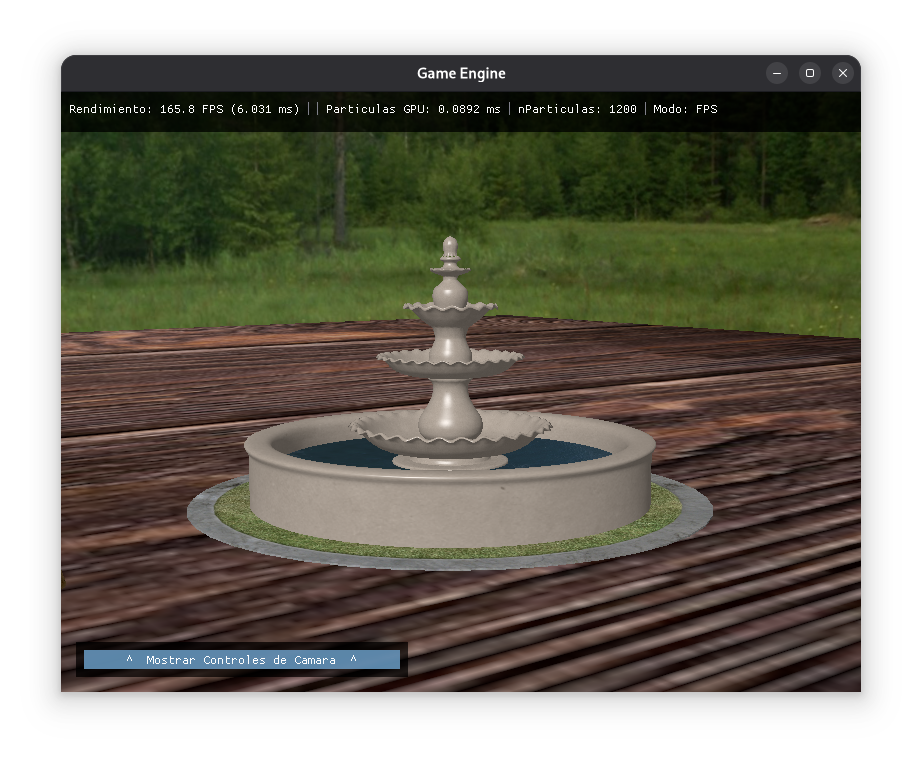
\includegraphics[width=1\textwidth]{Media/Desarrollo_6.png}
    \caption{Modelo de la fuente.}
    \label{fig:modFuente}
\end{figure}

El primer sistema que diseñamos fue la simulación de una fuente. La idea inicial era montar un entorno de pruebas sencillo para medir cómo se comportaban las trayectorias bajo fuerzas básicas. Se introdujo un modelo 3D de una fuente de piedra~\parencite{owenp88_fountain_2023} (Figura \ref{fig:modFuente}) y configuramos la lógica base en el archivo \texttt{GEAgua.cpp}. Como el objetivo era simplemente dar un resultado visual, se decidio no tratar con físicas de fluidos complejas como las basadas en las ecuaciones de Navier-Stokes y simulaciones GPU~\parencite{stam1999stable, akenine2018real} o colisiones detalladas con la piedra. Nos interesaba que el agua brotara con un impulso ascendente y la gravedad hiciera caer los puntos dibujando parábolas perfectas. Al final, lo logramos utilizando una cantidad de recursos notablemente inferior a la estimada inicialmente.

Para dar la sensacion de muchas gotas de agua sin lanzar muchisimas mas partículas había que engañar al ojo. En vez de usar puntitos sueltos, cargamos un sprite de alta resolución que ya traía el dibujo de una salpicadura rica~\parencite{pngwing_imagen_bnrwi} (Figura \ref{fig:texAgua}). Con esto ganamos muchísimo rendimiento. Un solo plano de textura representa visualmente el equivalente a cientos de microgotas calculadas individualmente. 

\begin{figure}[!htbp]
    \centering
    \tikz \node[draw, rounded corners=5pt, inner sep=0pt] {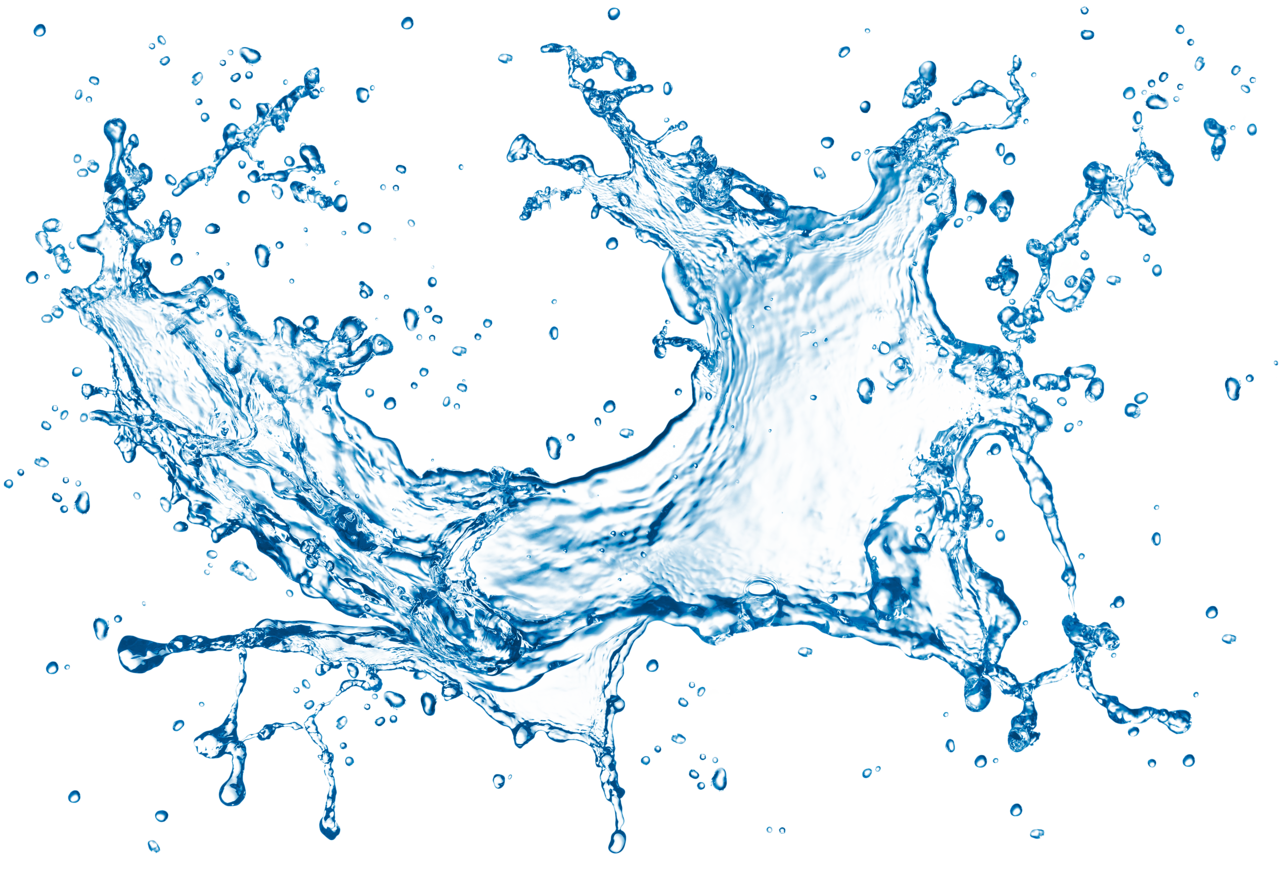
\includegraphics[width=0.4\textwidth]{Media/Desarrollo_1.png}};
    \caption{Textura del agua.}
    \label{fig:texAgua}
\end{figure}


\begin{figure}[!htbp]
    \centering
\begin{carbonbox}
void main() {
    uint index = gl_GlobalInvocationID.x; 
    if (index >= 100000) return;
    Particle p = particlesIn[index];
    p.currentTtl -= params.deltaTime;
    if (p.currentTtl <= 0.0) {
        p.currentTtl = p.ttl; 
        p.pos = params.emitterPos.xyz;
        // [Se calcula la velocidad inicial p.norm segun la formula de emision (Ec. (*\ref{eq:emision_agua}*))]
        p.color = params.startColor;
        p.size = params.startSize;
    } else {
        // [Se actualizan p.norm y p.pos segun la formula de integracion fisica (Ec. (*\ref{eq:integracion_agua}*))]
        float lifeFactor = 1.0 - (p.currentTtl / max(p.ttl, 0.001));
        p.color = mix(params.startColor, params.endColor, lifeFactor);
        p.size = mix(params.startSize, params.endSize, lifeFactor);
    }
    particlesOut[index] = p;
}
\end{carbonbox}
    \caption{Código fuente del sombreador \texttt{water.comp}.}
    \label{fig:water_comp}
\end{figure}

Todo el control matemático ocurre dentro de la GPU a través del shader de cómputo \texttt{water.comp} (véase la Figura~\ref{fig:water_comp}). Aquí la GPU lee el estado anterior de la partícula desde el búfer \texttt{particlesIn} y guarda los números nuevos en \texttt{particlesOut}. Organizamos la carga de trabajo de la gráfica en bloques de 256 hilos mediante \texttt{layout(local\_size\_x = 256)}. Cada hilo se ocupa de su propia gota. Como necesitábamos meter ruido al sistema para que los chorros no fueran idénticos, y en GLSL no hay funciones para tirar dados, improvisamos un algoritmo Hash a base de operaciones binarias XOR. Así conseguimos valores aleatorios de forma muy eficiente sin depender en nada del procesador del ordenador.           

El proceso matemático se evalúa de manera concurrente. En primera instancia, se sustrae el diferencial de tiempo (\texttt{deltaTime}) al ciclo de vida de la partícula (\texttt{currentTtl}). Si el elemento ha finalizado su ciclo vital (\texttt{currentTtl} $\le 0.0$), se reubica en la base del emisor. La dispersión direccional inicial se obtiene empleando coordenadas esféricas para generar ocho vectores fijos que rotan en función del tiempo, siguiendo el sistema expuesto en~(\ref{eq:emision_agua}):

\begin{equation}
    \label{eq:emision_agua}
    \begin{aligned}
        \theta_{\text{base}} &= \left(45^\circ \cdot (i \bmod 8) \cdot \frac{\pi}{180}\right) + (\text{time} \cdot v_{\text{rot}}) \\
        \phi &= 0.5236 + (\text{random}(i) - 0.5) \cdot 0.175 \\
        v_x &= \sin(\phi) \cdot \cos(\theta_{\text{base}}) \\
        v_y &= \cos(\phi) \\
        v_z &= \sin(\phi) \cdot \sin(\theta_{\text{base}})
    \end{aligned}
\end{equation}

Si el punto sigue vivo y flotando, se le aplica la gravedad utilizando el valor estándar ($g = 9.8$). Además, frenamos su avance hacia los lados aplicando un coeficiente de rozamiento ($R = 0.5$) para evitar que la fuente se desborde. Todo se integra directo con la ecuación~(\ref{eq:integracion_agua}):

\begin{equation}
    \label{eq:integracion_agua}
    \begin{aligned}
        v_y &= v_y - (g \cdot \Delta t) \\
        \vec{v}_{xz} &= \vec{v}_{xz} \cdot R^{\Delta t} \\
        \vec{p} &= \vec{p} + (\vec{v} \cdot \Delta t)
    \end{aligned}
\end{equation}

Toda esta parte de shaders está apoyada por la clase \texttt{GEAgua} en C++. El arranque aquí es muy estructurado. Definimos que cada partícula dure entre 2.0 y 3.5 segundos flotando, todo sacado de un motor \texttt{std::mt19937} inicializado como \texttt{static} para no perder ciclos de reloj tontos. A nivel estético, la gota pasa de azul eléctrico a transparente conforme pierde fuerza, y su tamaño se achica hasta desaparecer del todo.

El resultado salta a la vista. Las parábolas de agua que dibuja el sistema sobre el modelo de piedra resultan muy precisas (Figura~\ref{fig:resultadoAgua}). Usar texturas tan detalladas con mezcla aditiva fue un acierto enorme, ya que montamos un volumen líquido sin sobrecargar la tarjeta gráfica.

\begin{figure}[!htbp]
    \centering
    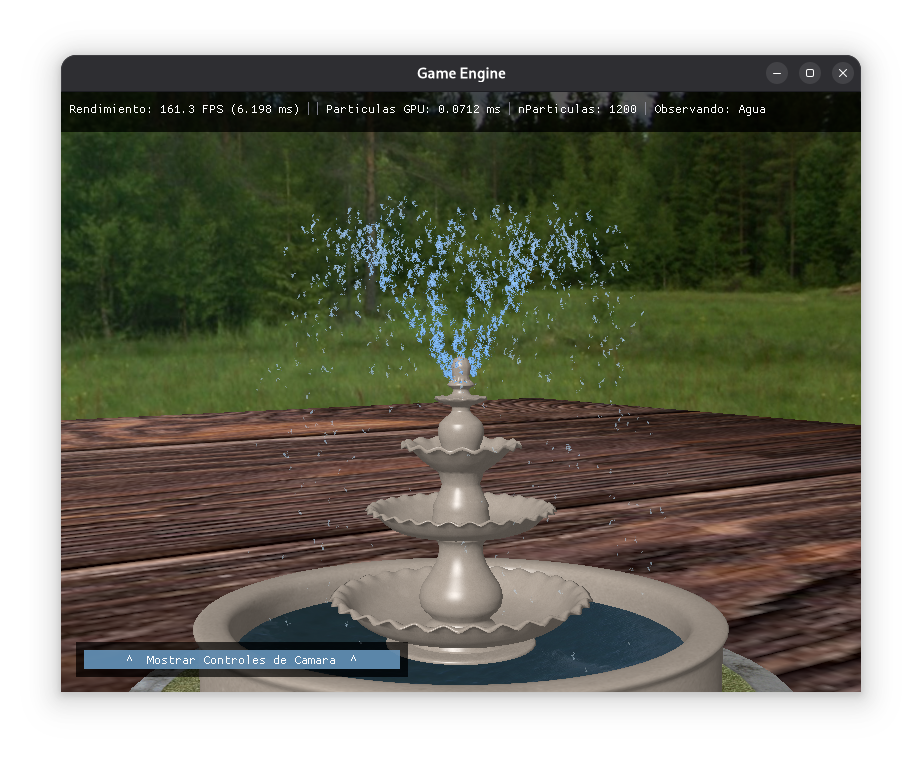
\includegraphics[width=1\textwidth]{Media/Conclusiones_3.png}
    \caption{Resultado visual final de la simulación del sistema de agua sobre la fuente.}
    \label{fig:resultadoAgua}
\end{figure}

\section{Fuego}

Teniendo el agua, pasamos a algo completamente distinto: el fuego. Lo curioso de este efecto es que la física opera al revés. No caen, sino que suben empujadas por la flotabilidad térmica. Para este escenario anclamos la simulación a un modelo tridimensional de troncos apilados~\parencite{hexmirelive_campfire_2026} (Figura \ref{fig:modHoguera}). Tampoco se implementaron cálculos termodinámicos complejos, el efecto lo conseguimos engañando a los ojos. Las llamas nacen anchas abajo y cortamos su tiempo de vida rápido para que se extingan antes de subir demasiado.

\begin{figure}[!htbp]
    \centering
    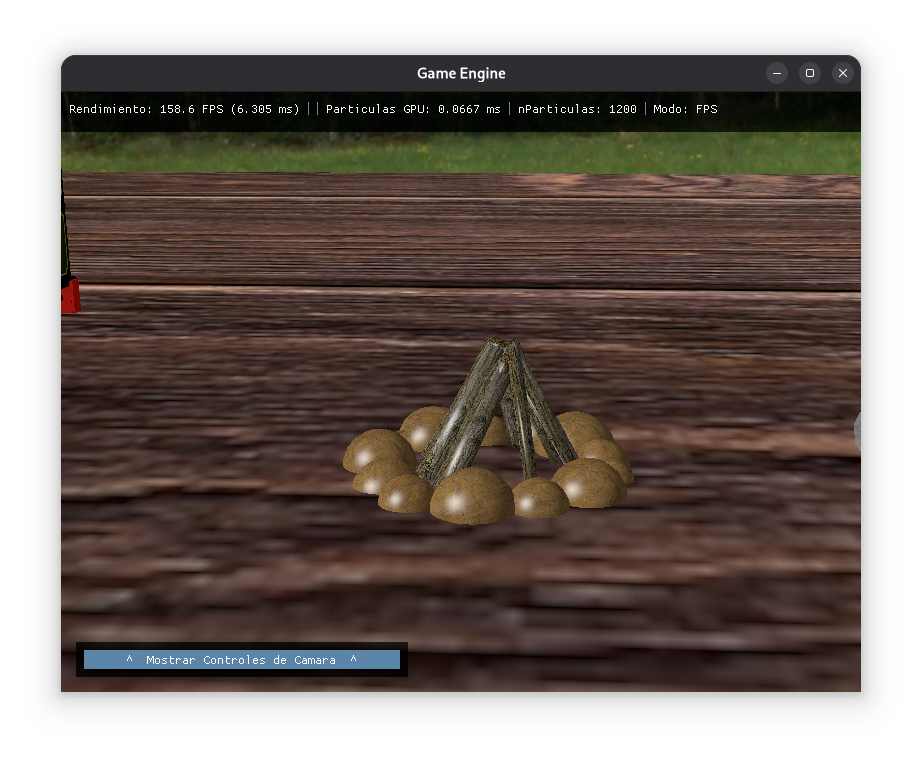
\includegraphics[width=1\textwidth]{Media/Desarrollo_5.png}
    \caption{Modelo de la hoguera.}
    \label{fig:modHoguera}
\end{figure}

Con el propósito de lograr una alta temperatura cromática, se descartaron \textit{sprites} de contornos nítidos y se empleó una textura difuminada~\parencite{Wolff_2013} (Figura \ref{fig:texFuego}). Gracias a la mezcla aditiva (\textit{additive blending}) configurada en la pipeline gráfica, las partículas superpuestas acumulan luminancia. Esto resulta en un núcleo incandescente de alta intensidad lumínica sobre los leños, evadiendo el alto coste computacional asociado a emisores de luz dinámicos y sombras en la escena tridimensional.

\begin{figure}[!htbp]
    \centering
    \tikz \node[draw, rounded corners=5pt, inner sep=0pt] {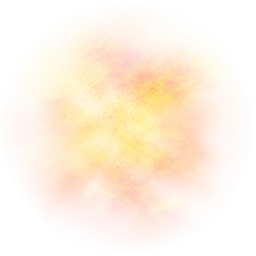
\includegraphics[width=0.4\textwidth]{Media/Desarrollo_2.png}};
    \caption{Textura del fuego.}
    \label{fig:texFuego}
\end{figure}


\begin{figure}[!htbp]
    \centering
\begin{carbonbox}
void main() {
    uint index = gl_GlobalInvocationID.x; 
    if (index >= 100000) return;
    Particle p = particlesIn[index];
    p.currentTtl -= params.deltaTime;
    if (p.currentTtl <= 0.0) {
        p.currentTtl = max(p.ttl, 0.1); 
        p.pos = params.emitterPos.xyz;
        // [Se aplica la dispersion circular en XZ (Ec. (*\ref{eq:distribucion_circulo_fuego}*)) y velocidad inicial a p.pos y p.norm]
        p.color = params.startColor;
        p.size = params.startSize;
    } else {
        float lifeFactor = 1.0 - (p.currentTtl / max(p.ttl, 0.001));
        bool esChispa = (index % 15 == 0);
        // [Se aplican fuerzas termicas, atraccion al centro y turbulencias a p.norm y p.pos]
        p.color = mix(params.startColor, params.endColor, lifeFactor);
        // [Se calcula el tamano del fuego con atenuacion polinomial (Ec. (*\ref{eq:atenuacion_tamano_fuego}*)) en p.size]
    }
    particlesOut[index] = p;
}
\end{carbonbox}
    \caption{Código fuente del sombreador \texttt{fire.comp}.}
    \label{fig:fire_comp}
\end{figure}


Todo el control de temperatura simulada se gestiona en el shader de computación \texttt{fire.comp} (véase la Figura~\ref{fig:fire_comp}). Cuando las partículas de la base agotan su vida, se regeneran en la base, pero con un matiz clave. El fuego no puede salir de un solo punto fino, así que se distribuye su origen de forma circular en el plano horizontal $XZ$. Para evitar su concentración en el centro, se fuerza una distribución aplicando la raíz cuadrada al calcular el radio, según esta fórmula~(\ref{eq:distribucion_circulo_fuego}):

\begin{equation}
    \label{eq:distribucion_circulo_fuego}
    \begin{aligned}
        \theta &= \text{random}(i) \cdot 2\pi \\
        r &= \sqrt{\text{random}(i + 1000)} \cdot \text{randomness} \cdot 0.5
    \end{aligned}
\end{equation}

A las partículas activas en ascenso se les aplican tres fuerzas diferentes. En primer lugar, una fuerza térmica que las desplaza verticalmente. Simultáneamente, dado que las llamas reales se estrechan en la punta debido a la convección térmica, se empujan levemente las partículas hacia el centro de la fogata. Como añadido final, se suma la característica turbulencia de una llama. Esto se consigue de forma eficiente, aplicando funciones seno y coseno sobre los ejes $X$ y $Z$. Se introducen variables de tiempo y semilla aleatoria por hilo para romper cualquier patrón geométrico discernible.

Como añadido estético que aporta gran riqueza visual, se configuró que una de cada quince partículas (usando la operación \texttt{index \% 15 == 0}) se transforme en una chispa voladora. Estos elementos menores no siguen la dinámica de grupo. Se elimina su tendencia hacia el centro para permitir su dispersión lateral, y se les añaden trayectorias elípticas caóticas. Simulan con fidelidad fragmentos incandescentes.





Para que el efecto de quemado resulte natural, el color transita del amarillo intenso al rojo con alta transparencia. El tamaño no disminuye progresivamente. Se ha diseñado la simulación para que la llama mantenga su volumen durante la mayor parte de su ciclo y se reduzca de forma drástica justo antes de desaparecer, empleando para ello una función matemática polinomial eficiente~(\ref{eq:atenuacion_tamano_fuego}):

\begin{equation}
    \label{eq:atenuacion_tamano_fuego}
    \text{factorTama\~no} = 1.0 - (\text{lifeFactor})^2
\end{equation}

En la capa de control de la CPU se utiliza la clase \texttt{GEFuego}. Para conseguir un arranque explosivo, se emiten las partículas directamente con un vector de dirección vertical~(\ref{eq:normal_fuego_cpp}):

\begin{equation}
    \label{eq:normal_fuego_cpp}
    \vec{n} = (0.0, 1.0, 0.0)
\end{equation}

El empuje ascendente base se establece mediante una fuerza constante de $2.0$. El dinamismo de la simulación, que previene una ascensión excesivamente homogénea o rectilínea, reside en la asignación del parámetro de dispersión \texttt{randomness = 2.0f}. Desde la GPU, este coeficiente perturba lateralmente las componentes de velocidad de cada hilo de ejecución de manera pseudoaleatoria, emulando la turbulencia térmica característica presente en la hoguera (Figura~\ref{fig:resultadoFuego}).

\begin{figure}[!htbp]
    \centering
    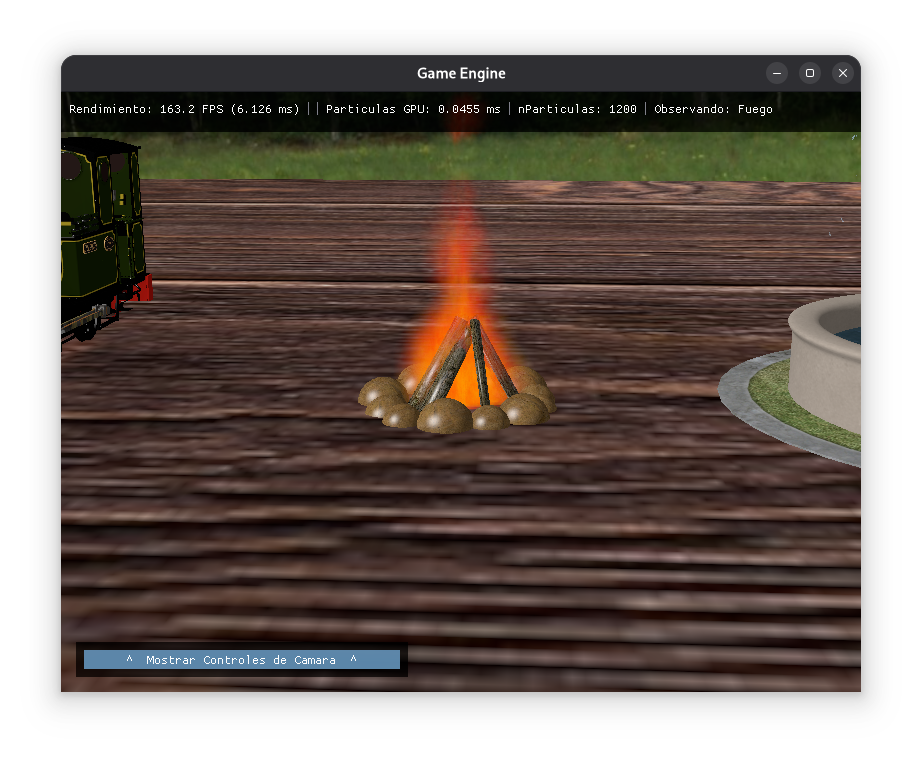
\includegraphics[width=1\textwidth]{Media/Conclusiones_2.png}
    \caption{Resultado visual final del sistema de fuego en el entorno de la hoguera.}
    \label{fig:resultadoFuego}
\end{figure}

\section{Humo}

\begin{figure}[!htbp]
    \centering
    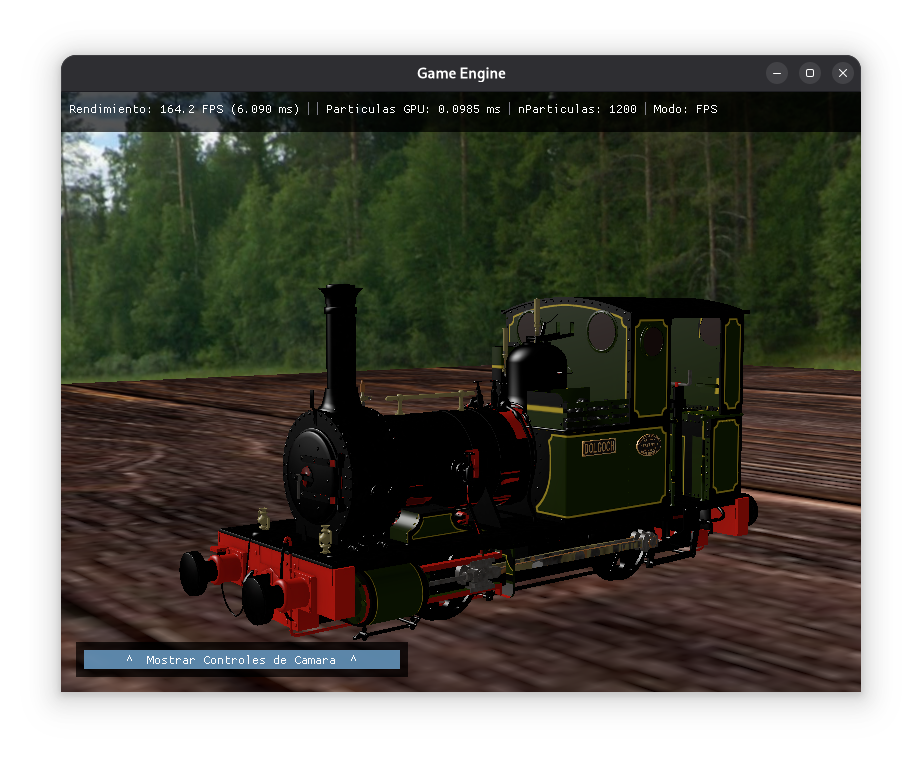
\includegraphics[width=1\textwidth]{Media/Desarrollo_4.png}
    \caption{Modelo del tren.}
    \label{fig:modTren}
\end{figure}


La simulación del humo fue la última en implementarse, requiriendo sus propias reglas físicas. A diferencia de la fuerza bruta del fuego, las nubes de humo crecen lento y duran mucho tiempo dando vueltas en pantalla. Usamos la clásica técnica de \textit{alpha blending} para la transparencia. Con esto, las partículas grises se montan unas sobre otras y borran con mucha suavidad el fondo del escenario. Se ven como columnas densas con mucho peso. 

Para anclar la simulación, decidimos poner una locomotora antigua~\parencite{planeharmony389_dolgoch_2026} (Figura \ref{fig:modTren}). Su chimenea era el agujero perfecto para probar chorros direccionados de humo grueso y ver cómo el volumen ganaba escala al subir hacia el cielo.

\vspace{4\baselineskip}

\begin{figure}[!htbp]
    \centering
    \tikz \node[draw, rounded corners=5pt, inner sep=0pt] {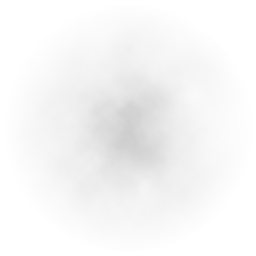
\includegraphics[width=0.4\textwidth]{Media/Desarrollo_3.png}};
    \caption{Textura del humo.}
    \label{fig:texHumo}
\end{figure}


La elección de la textura del humo resultó fundamental. Dada su escalabilidad progresiva, cualquier imperfección o delineado provocaría anomalias visuales, motivo por el que se utilizó una distribución gaussiana opaca carente de contornos definidos~\parencite{Wolff_2013} (Figura \ref{fig:texHumo}). La superposición volumétrica de estas texturas enmascara la geometría plana de las primitivas, originando una representación gaseosa y suave empleando un mínimo número de partículas.


El algoritmo de control dinámico se encuentra en el shader \texttt{smoke.comp} (véase la Figura~\ref{fig:smoke_comp}). Al resetear el ciclo de vida de los puntos, la chimenea los emite con una componente de aceleración vertical y una leve dispersión horizontal tridimensional aleatoria, generando una emisión cónica realista.

\begin{figure}[!htbp]
    \centering
\begin{carbonbox}
void main() {
    uint index = gl_GlobalInvocationID.x; 
    if (index >= 100000) return;
    Particle p = particlesIn[index];
    p.currentTtl -= params.deltaTime;
    if (p.currentTtl <= 0.0) {
        p.currentTtl = max(p.ttl, 0.1); 
        p.pos = params.emitterPos.xyz;
        // [Se aplica la dispersion inicial en abanico 3D a la velocidad p.norm]
        p.color = params.startColor;
        p.size = params.startSize;
    } else {
        p.norm += params.force.xyz * params.deltaTime;
        p.pos += p.norm * params.deltaTime;
        // [Se aplica la perturbacion de la brisa tipo remolino (Ec. (*\ref{eq:remolino_humo}*)) sobre p.pos.xz]
        float lifeFactor = 1.0 - (p.currentTtl / max(p.ttl, 0.001));
        p.color = mix(params.startColor, params.endColor, lifeFactor);
        p.size = mix(params.startSize, params.endSize, lifeFactor);
    }
    particlesOut[index] = p;
}
\end{carbonbox}
    \caption{Código fuente del sombreador \texttt{smoke.comp}.}
    \label{fig:smoke_comp}
\end{figure}

A lo largo de su ascensión, las partículas están sujetas a una fuerza de sustentación constante. Para modelar turbulencias atmosféricas sutiles se descartó el uso de mapas de ruido procedimental tridimensional tipo Perlin o Simplex~\parencite{perlin1985an, perlin2002improving} debido a su carga sobre la GPU. En contrapartida, se optó por perturbar la posición horizontal empleando funciones armónicas. Alterando la frecuencia de oscilación en los ejes $X$ ($2.0$) y $Z$ ($1.5$), se fuerza a las partículas a describir trayectorias helicoidales y elípticas en su desplazamiento, según se modela en la ecuación~(\ref{eq:remolino_humo}):

\begin{equation}
    \label{eq:remolino_humo}
    \begin{aligned}
        \text{swirl}_x &= \sin(P_y \cdot 0.5 + \text{time} \cdot 2.0) \cdot \text{randomness} \\
        \text{swirl}_z &= \cos(P_y \cdot 0.5 + \text{time} \cdot 1.5) \cdot \text{randomness}
    \end{aligned}
\end{equation}

El toque final lo da la clase de control principal \texttt{GEHumo}. Para que el efecto sea de nube densa, las partículas empiezan con un tamaño reducido de $1.5$ y se expanden considerablemente, alcanzando una escala de $15.0$ cuando van a desaparecer de pantalla. Al sumarle a esto un ciclo de vida prolongado (entre 2.0 y 6.0 segundos) y un color que arranca en gris cerrado para morir en una transparencia negra absoluta, el resultado es justo lo que buscábamos.                            

La locomotora expulsa una columna negra gigantesca que se va disipando según choca contra la atmósfera, como se observa en la Figura~\ref{fig:resultadoHumo}. El efecto está plenamente conseguido apoyándose exclusivamente en modelos matemáticos.

\begin{figure}[!htbp]
    \centering
    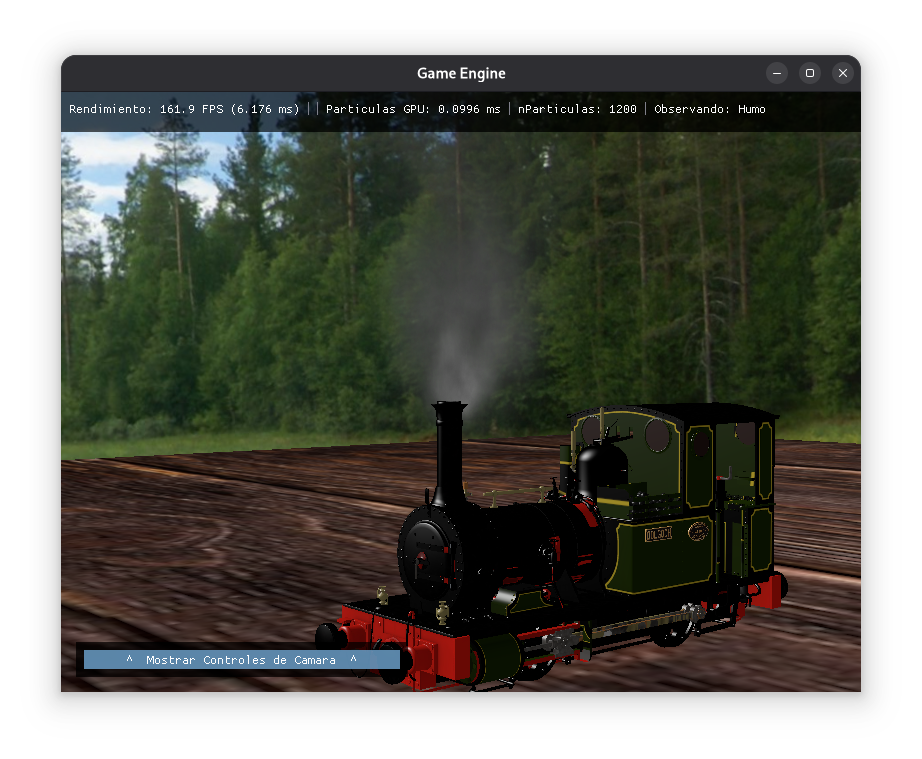
\includegraphics[width=1\textwidth]{Media/Conclusiones_1.png}
    \caption{Humo saliendo de la chimenea de la locomotora.}
    \label{fig:resultadoHumo}
\end{figure}